\let\negmedspace\undefined
\let\negthickspace\undefined
\documentclass[journal]{IEEEtran}
\usepackage[a5paper, margin=10mm, onecolumn]{geometry}
\usepackage{lmodern} % Ensure lmodern is loaded for pdflatex
\usepackage{tfrupee} % Include tfrupee package

\setlength{\headheight}{1cm} % Set the height of the header box
\setlength{\headsep}{0mm}     % Set the distance between the header box and the top of the text

\usepackage{gvv-book}
\usepackage{gvv}
\usepackage{cite}
\usepackage{amsmath,amssymb,amsfonts,amsthm}
\usepackage{algorithmic}
\usepackage{graphicx}
\graphicspath{{./figs/}}
\usepackage{textcomp}
\usepackage{xcolor}
\usepackage{txfonts}
\usepackage{listings}
\usepackage{enumitem}
\usepackage{mathtools}
\usepackage{gensymb}
\usepackage{comment}
\usepackage[breaklinks=true]{hyperref}
\usepackage{tkz-euclide} 
\usepackage{listings}
\usepackage{gvv}                                        
\def\inputGnumericTable{}                                 
\usepackage[latin1]{inputenc}                                
\usepackage{color}                                            
\usepackage{array}                                            
\usepackage{longtable}                                       
\usepackage{calc}                                             
\usepackage{multirow}                                         
\usepackage{hhline}                                           
\usepackage{ifthen}                                           
\usepackage{lscape}
\usepackage{circuitikz}
\tikzstyle{block} = [rectangle, draw, fill=blue!20, 
text width=4em, text centered, rounded corners, minimum height=3em]
\tikzstyle{sum} = [draw, fill=blue!10, circle, minimum size=1cm, node distance=1.5cm]
\tikzstyle{input} = [coordinate]
\tikzstyle{output} = [coordinate]
\begin{document}
\bibliographystyle{IEEEtran}
\vspace{3cm}
\title{4.7.47}
\author{EE25BTECH11050-Hema Havil}
	\maketitle
	% \newpage
	% \bigskip
	{\let\newpage\relax\maketitle}
	
	\renewcommand{\thefigure}{\theenumi}
	\renewcommand{\thetable}{\theenumi}
	\setlength{\intextsep}{12pt} % Space between text and floats
	
	\numberwithin{equation}{enumi}
	\numberwithin{figure}{enumi}
	\renewcommand{\thetable}{\theenumi}
	
	\textbf{Question}:\\
    
         The foot of perpendiculars from the point (2, 3) on the line $y = 3x + 4$ is given by
         
         \solution \\
         Let the given point be P=(2,3) and let the foot of perpendicular be Q and let the given line be written as,
         \begin{align}
             \vec{n}^T\vec{x}=c
         \end{align}
         where\\
         \begin{align*}
             \vec{n} = \myvec{3\\-1} \\ c=-4
         \end{align*}
         then Q is a point on the line, Hence it satisfies the line equation
         \begin{align}
             \vec{n}^T\vec{Q}=c
         \end{align}
         Let $\vec{m}=(a,b)$ be the direction vector of the line 
         \begin{align}
             \vec{m}^T\vec{n}=0
         \end{align}
         \begin{align}
             \myvec{a\;b}\myvec{3\\-1}=0
         \end{align}
         \begin{align}
             3a=b
         \end{align}
         \begin{align}
             \vec{m}=\myvec{1\\3}
         \end{align}
         Then m is perpendicular to direction vector along PQ\\
         \begin{align}
             \vec{m}^T(\vec{Q}-\vec{P})=0
         \end{align}
         \begin{align}
             \vec{m}^T\vec{Q}=\vec{m}^T\vec{P}
         \end{align}
         from equation (0.2) and (0.8) we can write 
         \begin{align}
             \myvec{\vec{m}\;\;\vec{n}}^T\vec{Q}=\myvec{\vec{m}^T\vec{P}\\c}
         \end{align}
         We can find the value of $\vec{m}^T\vec{P}$
         \begin{align}
             \vec{m}^T\vec{P}=\myvec{1\;3}\myvec{2\\3}=\myvec{2+9}=\myvec{11}
         \end{align}
         From this we can find Q, substitute values in (0.9)
         \begin{align}
             \myvec{1\;\;\;\;3\\3\;-1}^T\vec{Q}=\myvec{11\\-4}
         \end{align}
         \begin{align}
             \myvec{1\;\;\;\;3\\3\;-1}\vec{Q}=\myvec{11\\-4}
         \end{align}
         This can be solved using augmented matrix and let the augmented matrix be A
         \begin{align}
             \vec{A}=\myvec{1\;\;\;\;3\;\;\;\;11\\3\;-1\;-4}
         \end{align}
         $R_2\rightarrow{R_2-3R_1}$
         \begin{align}
             \vec{A}=\myvec{1\;\;\;\;3\;\;\;\;11\\0\;-10\;-37}
         \end{align}
         $R_1\rightarrow{R_1+\frac{3}{10}R_2}$ \hspace{1cm}
         $R_2\rightarrow{\frac{-1}{10}R_2}$
         \begin{align}
             \vec{A}=\myvec{1\;\;\;\;0\;\;\;\;\frac{-1}{10}\\\\0\;\;\;1\;\;\;\;\frac{-37}{10}}
         \end{align}
         Therefore from (0.15) the value of Q is
         \begin{align}
             \vec{Q}=\myvec{\frac{-1}{10}\\\\ \frac{-37}{10}}
         \end{align}
         \begin{figure}
             \centering
             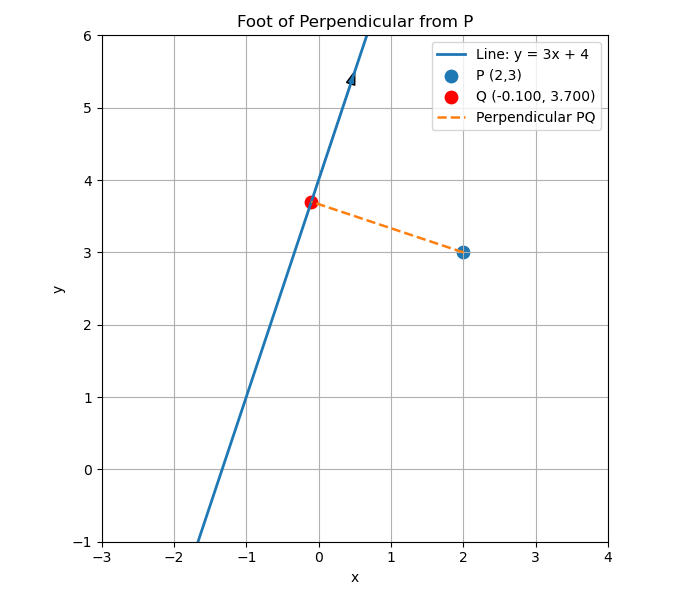
\includegraphics[width=0.7\columnwidth]{figs/fig1.png}
             \caption{Plot for foot of perpendicular of P}
             \label{fig1}
         \end{figure}
    
         
\end{document}

